\documentclass{article}
\usepackage{gensymb, amsmath, float, graphicx, epstopdf}
\restylefloat{table}
\usepackage[margin=0.75in]{geometry}
\begin{document}

\title{Lab Write-up 4: Shielded-Loop Resonators}
\author{Michael Shen}
\maketitle


\section{Finding the Resonant Frequency}

\subsection{Measured Data}

\begin{table}[H]
\centering
\begin{tabular}{|l|l|l|}
\hline
Loop & $f_0$ & $\vert\Gamma^{\prime}_{in}\vert$ \\ \hline
5 cm &  &  \\ \hline
9 cm &  &  \\ \hline
\end{tabular}
\end{table}

\subsection{Questions}

\begin{enumerate}
	\item 
	\item 
	\item 
\end{enumerate}


\section{De-embedding the Feedline}

\subsection{Measured Data}
\begin{table}[H]
\centering
\begin{tabular}{|l|l|l|l|}
\hline
Loop & $\vert\Gamma^{\prime}_{in}\vert$ & $\vert\Gamma^{\prime}_{in}\vert$ at $f_0$ - 2MHz & $\vert\Gamma^{\prime}_{in}\vert$ at $f_0$ + 2MHz \\ \hline
5 cm &  &  &  \\ \hline
9 cm &  &  &  \\ \hline
\end{tabular}
\end{table}

\subsection{Analysis}
\begin{enumerate}
	\item 
	\item 
	\item 
	\item 
	\item 
\end{enumerate}

\subsection{Questions}
\begin{enumerate}
	\item 
	\item 
\end{enumerate}


\section{Finding R, L, and C}

\subsection{Measured Data}
\begin{table}[H]
\centering
\begin{tabular}{|l|l|l|l|}
\hline
Loop & R & L & C \\ \hline
5 cm &   &   &  \\ \hline
9 cm &   &   &  \\ \hline
\end{tabular}
\end{table}

\subsection{Analysis}

\begin{enumerate}
	\item
	\item
\end{enumerate}

\subsection{Questions}

\begin{enumerate}
	\item 
	\item 
	\item 
\end{enumerate}

%\section{Figures and Images}
%\begin{figure}[H]
%    \centering
%    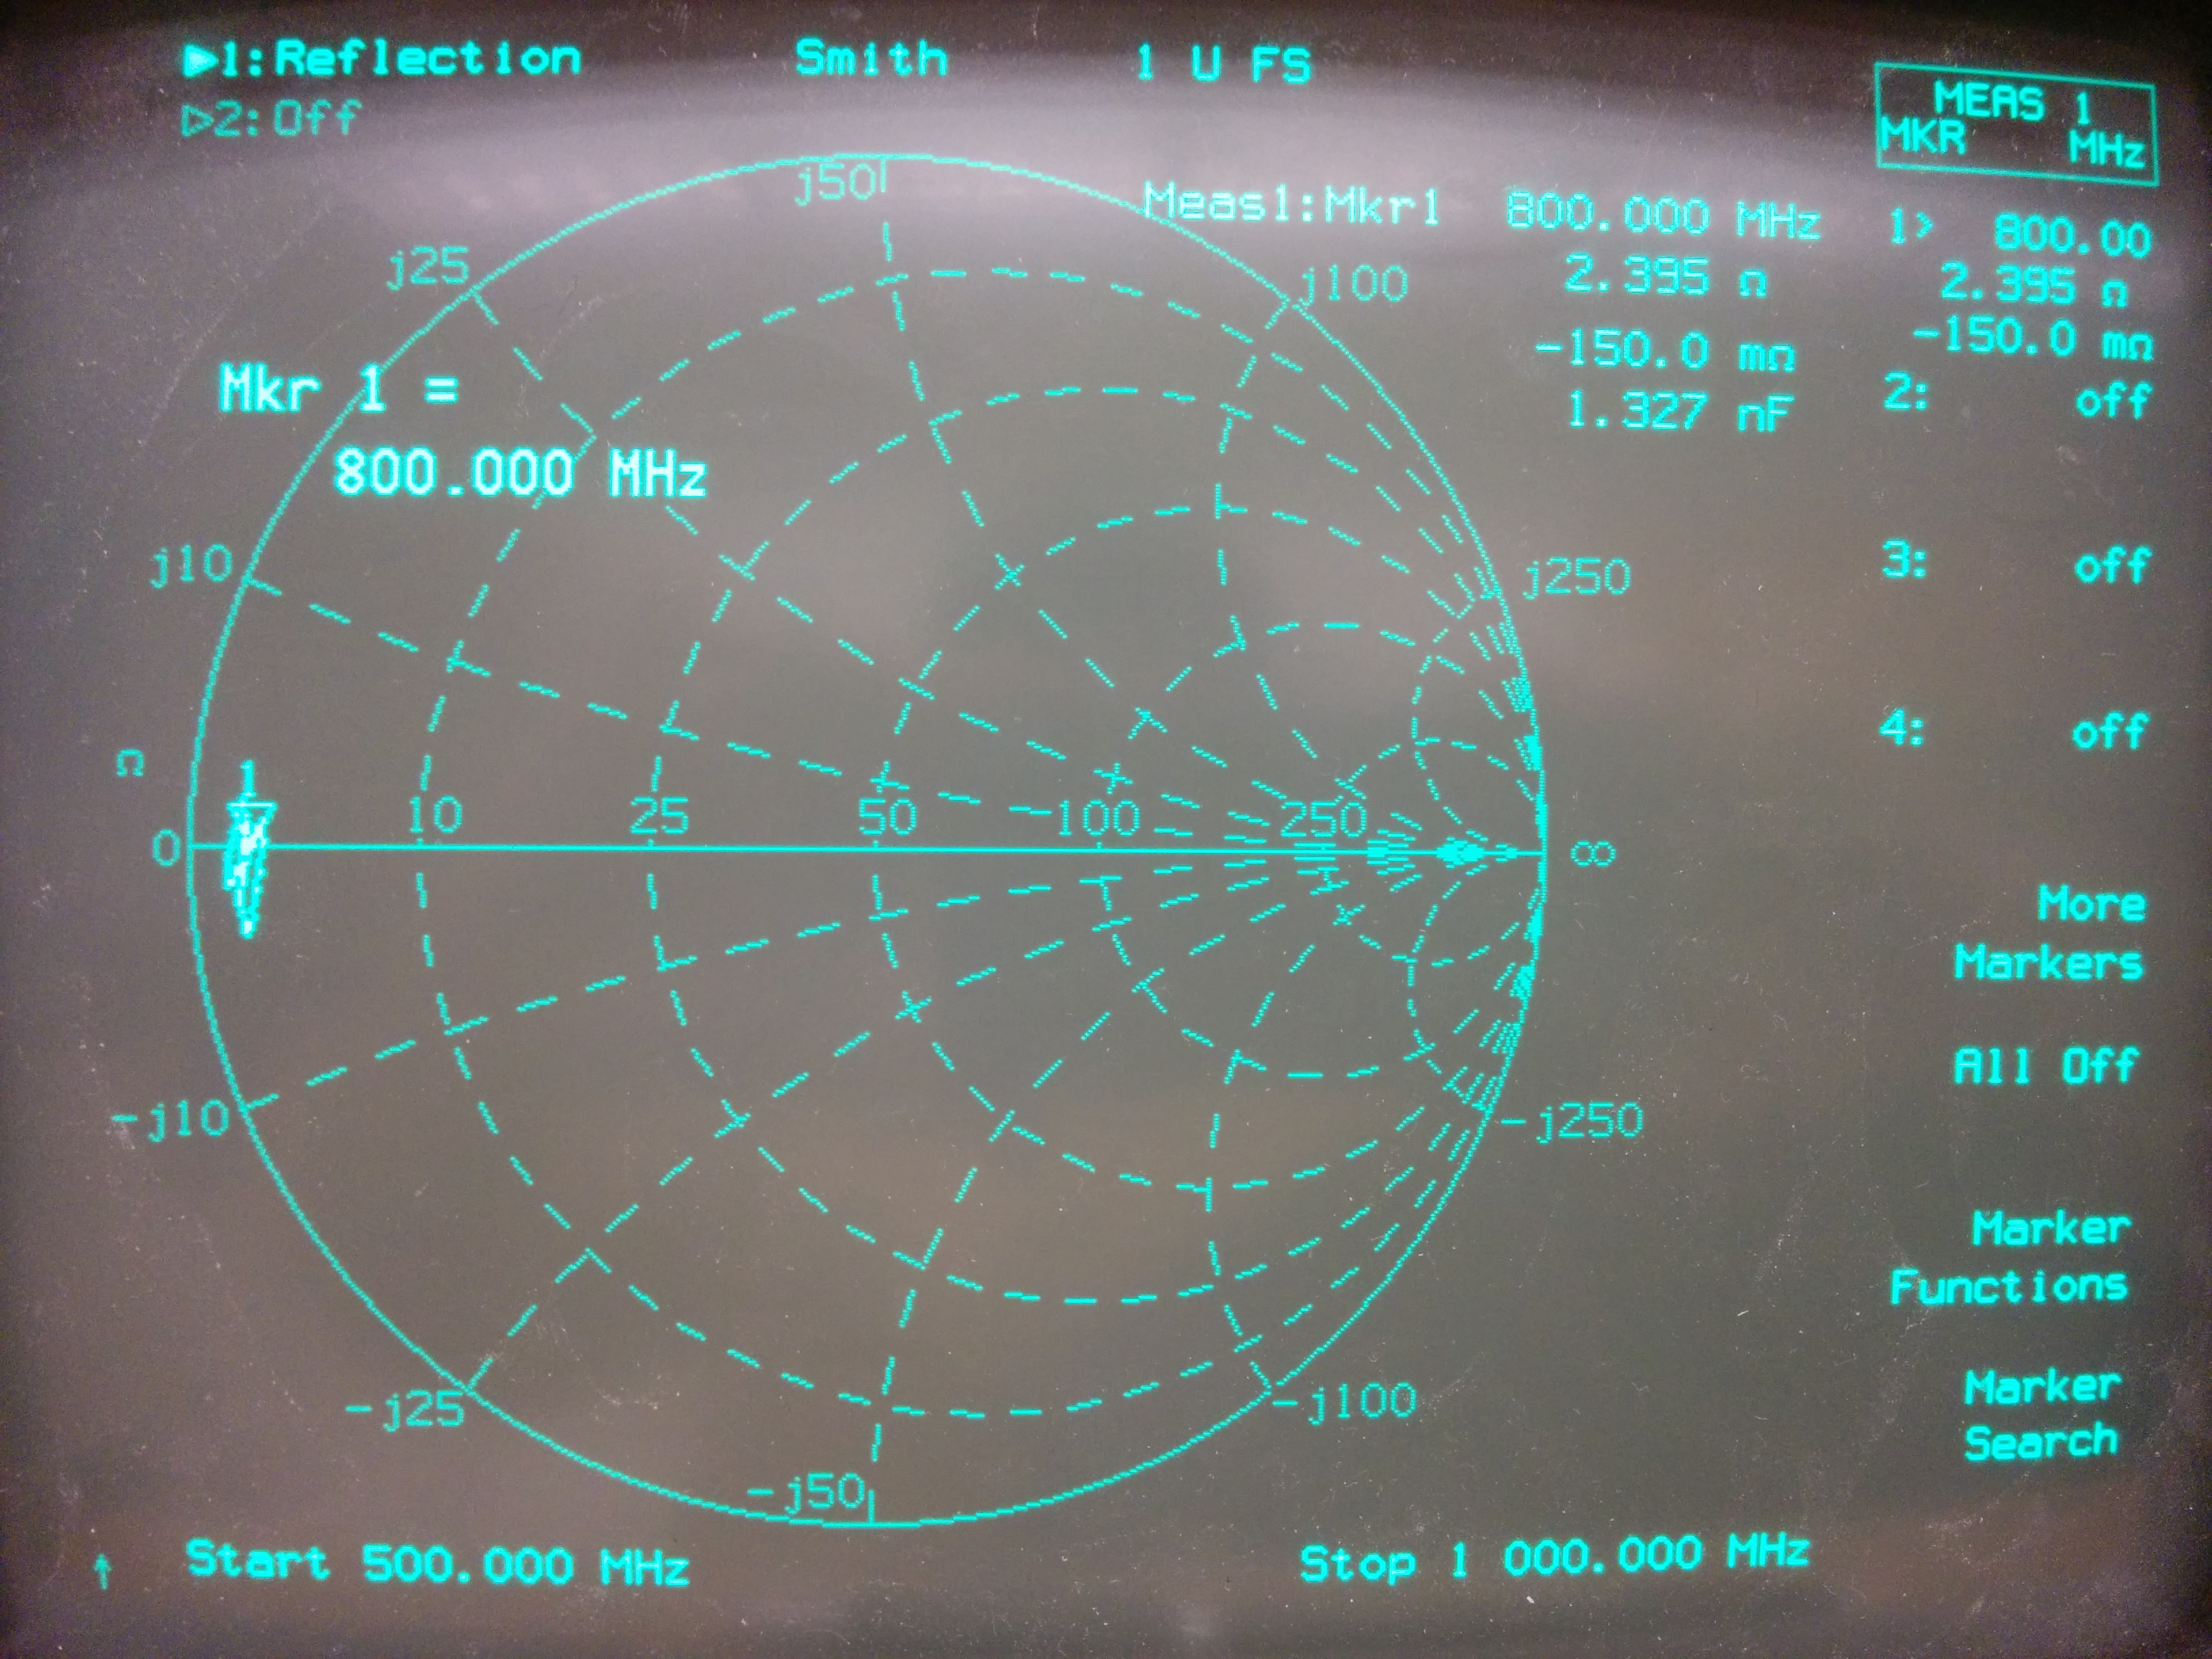
\includegraphics[width=0.8\textwidth]{./Images/251.jpg}
%    \caption{Point-like response for a lossless line}
%\end{figure}

\end{document}